\section{Introduction} \label{intro}

Sleep is considered to be ubicuitous and necessary in so far as it was observed in most animal models.

In vertebrate, electrophysiological recordings, in particular, \gls{eeg}, but also \gls{emg}
Classically, activity has been classified in several discrete \emph{vigilance states}...

In rodents, three vigilance states are usually defined on the basis of \gls{eeg} and \gls{emg} (fig.~\ref{fig:sleep_description}).
When awake (WAKE), an animal tends to have a high muscular activity which translates as a high amplitude in the \gls{emg} and a relatively low amplitude
\gls{eeg} domitated by oscilations of frequency between six and ten hertz often refered as theta waves.
In contrast, \gls{nrem} sleep, also called slow wave sleep is a period of muscular inactivity (low \gls{emg}) dominated by slow oscilations (below 4Hz) of high amplitude named delta waves.
Finally, \gls{rem} sleep is characterised by a complete lack of muscular activity (atony) and an \gls{eeg} activity very similar to the awake state.
\gls{rem} sleep is the least prevalent of all three stages, and generally represents less that  20\% of all sleeping time.

\begin{figure}[h!]
  \centering   
    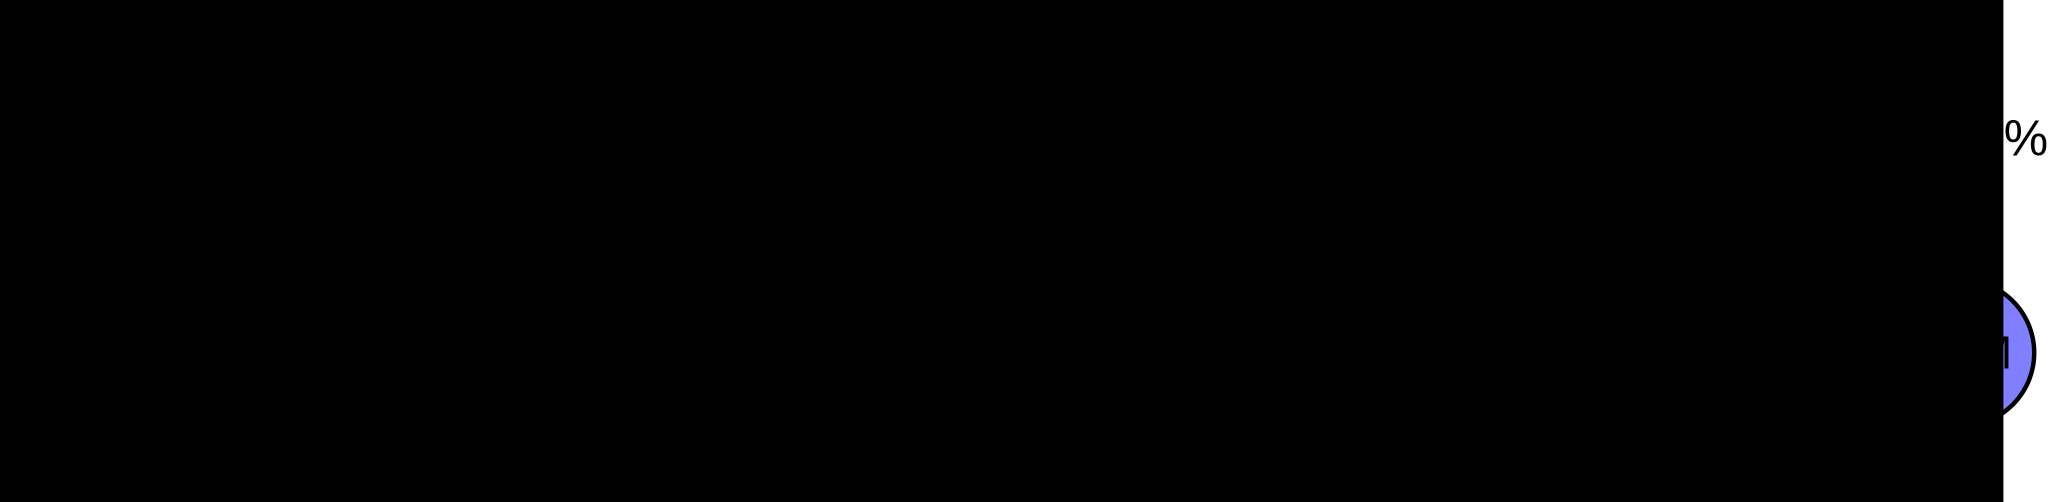
\includegraphics[width=0.95\textwidth]{figures/sleep_description.pdf}
  \caption{\ctit{Structural description of sleep stages.}
  \textbf{A}: Characteristics of the three vigilance states: \gls{nrem}, \gls{rem} and wakefulness.
  Typically, frequency and amplitude of the \acrfull{eeg}, and amplitude of the \acrfull{emg} are used by experts to infer vigilance state.
  The frequency ranges and prevalences are approximate values for healthy adult animals in normal conditions.
  Each wave shows a representative five second epoch with high signal to noise ratio.
  \textbf{B}: Empirical transition probabilities between consecutive five second epochs. 
  The width of the arrow is proportional to transition probability.
  Values have been computed from the 12 recordings used in this study.
  Probabilities of remaining in each state are implied.
  \label{fig:sleep_description}
  }
\end{figure}





Although this definitions appear straigthforward, in practice, many cases are ambigous. 
For instance, it is difficult to characterise transitions between two states.
In addition, there are many sources of variability including how surgery was performed by the experimenter,
 the type of recorder used and inter-animal variability.
The quality of the aquisition can also be made considerably worst by noisy  signals or when the presence of artefacts.
For these reasons, sleep scoring, the attribution of discrete vigilence states to electrophysiological time series, is traditionnally performed by trained human experts.
This task is very time consuming; several hours of work have been reported in order to score 24h of recording.
This severely limits data throughput and human subjectivity is likely to introduce systematic bias. 
Indeed, it is expected that scoring will be perfomred differently by each expert, making result difficult to reproduce independently.
Often, two experts score the same time data, in order to ensure satifying aggreement. In general, the inter-human aggrement is important \citationneeded{}.
It can however be argued that experts most likely work in the same laboratory and trained one another, or were trained by the same third person.
In this context, aggremment between experts does not account for the variability between communities of researchers, and cannot be used to assess reproducibility.

In order to overcome both speed and subjectivity limitations, efforts have been directed towards automation of sleep scoring.
However, there is little addoption of automatic method and very few available implementations in the form of software that biologists could use.
Typically, two different approches have been followed: unsupervided or supervided learning.

Unsupervised learning has the advantage of making no assumption about the nature of the different vigilence states.
Therefore, this approach can lead to the discovery of truely new states.
One issue is that the choice of the variables used for clustering will be critical.
Often, variables such as frequency domain variables chosen in order to generate clusters that will match human defined clusters.
In addition, unsupervided methods may lack robustness in so far as the cannot easily include covariates explaining, for instance, variability between recording equipments.


Another approach is to assume human annotations are in general biologically relevant and consistant, and to use supervided learning teachniques.
Of course, if human decisions were baised, such a method may reproduce this biais.
However, a vast corpus of experimental work has provided hypothesis about function of these states.
Building a classifier that would produce a consensual prediction of vigilence states could be seen as an attempt to formalised and rationnalise the definition of such states.
This could improving future research without denying decades of sleep neurobiology. 

Many supervised learning techniques ranging from SVM, ANNs, to HMMs have been investigated.
In general, the first step is to compute features on subsequent segments, know as epochs, of annotated electrophysiological signals.
Then, the relation between the response variable(annotation) and the independent variables (features) can be modeled.
Either epochs are considered to be independent from one another or time-dependent structures are explicitely modeled (\eg{} HMMs).

Recently, promissing results were obtained for scoring human sleep stages by performing an exhaustive feature extraction including variables resulting from discrete wavelet decomposition.
Then, the authors compared several classifiers and found that random forest were the most accurate.

The study herein bases itself on these promissing results by computing an even larger number of features.
An important addition is the computation of time-aware features which significantly improved accuracy.
In addition, rigourous startified cross-validation procedure and comparisons of sleep structure were performed.

In order to pave the way to an implementation of an ubicuitous sleep scoring software.
\pr, a new \py{} package was also build to facilitate efficient feature extraction. 
This new package is here demonstated to be significantly more performant than preexisting implementation.

